\documentclass[12pt]{article}
\usepackage{sbc-template}
\usepackage{graphicx,url}
\usepackage[utf8]{inputenc}
\usepackage[brazil]{babel}
\usepackage{booktabs}
\usepackage{array}
\usepackage{float}
\usepackage{iftex}
% O modelo SBC usa Times. No XeLaTeX/Tectonic, configurar as fontes
% explicitamente evita substituição silenciosa por Latin Modern.
\ifPDFTeX\else
  \usepackage{fontspec}
  \IfFontExistsTF{Times New Roman}{\setmainfont{Times New Roman}}{\setmainfont{TeX Gyre Termes}}
  \IfFontExistsTF{Arial}{\setsansfont{Arial}}{\setsansfont{TeX Gyre Heros}}
  \IfFontExistsTF{Courier New}{\setmonofont{Courier New}}{\setmonofont{TeX Gyre Cursor}}
\fi

% Primeira versão de trabalho. Imagens e resultados pendentes são indicados
% nos espaços próprios; consultar LEIA-ME.md antes de produzir a versão final.
\title{CLACK: Automatizando o Fluxo de Acesso Acadêmico\newline Via Trancas Inteligentes}

\author{William Palhares Meireles\inst{1}, Vinicius Bittencourt da Silva\inst{1},\\
Karine Nóra Dias\inst{1}}

\address{Instituto Federal Sul-rio-grandense (IFSul)\\
Campus Sant'Ana do Livramento -- RS -- Brasil
\email{williammeireles.sl007@academico.ifsul.edu.br}
\email{viniciusbittencourt@ifsul.edu.br}
\email{karinedias@ifsul.edu.br}}

\begin{document}
\maketitle

\begin{abstract}
This paper presents Clack, a prototype for managing access to academic rooms through RFID locks and a web application. The solution combines an ESP32, an RFID reader, an actuator, and a local server responsible for user permissions and event records. The lock stores permissions locally and synchronizes events when communication is available. An accelerated load experiment with 50 simulated locks generated 3,060 requests in 60.04 seconds, with no reported errors and all 1,000 expected events recorded. The results support the feasibility of the tested software scenario; physical durability, prolonged operation, security improvements, and evaluation with users remain necessary.
\end{abstract}

\begin{resumo}
Este artigo apresenta o Clack, protótipo de controle de acesso a salas acadêmicas por trancas RFID e aplicação web. A solução reúne ESP32, leitor RFID, atuador e servidor local para gerenciamento de permissões e registro de eventos. A tranca mantém permissões localmente e sincroniza eventos quando há comunicação. Em um ensaio acelerado com 50 trancas simuladas, foram realizadas 3.060 requisições em 60,04 segundos, sem erros registrados e com os 1.000 eventos esperados. Os resultados demonstram o funcionamento do cenário de software testado; resistência física, operação prolongada, melhorias de segurança e avaliação com usuários ainda necessitam de investigação.
\end{resumo}

\noindent\textbf{Palavras-chave:} controle de acesso; RFID; ESP32; internet das coisas; servidor web.

\section{Introdução}

O acesso a salas de aula, laboratórios e outros ambientes institucionais envolve a autorização de pessoas e o acompanhamento do uso dos espaços. Quando esse processo depende da retirada e devolução de chaves físicas, a portaria e os usuários precisam coordenar a entrega das chaves e seus respectivos registros. No contexto do Instituto Federal Sul-rio-grandense (IFSul), Campus Sant'Ana do Livramento, o projeto Clack foi motivado pela possibilidade de apoiar essa rotina com identificação eletrônica e gestão centralizada, mantendo a portaria informada sobre as atividades registradas.

A proposta integra uma tranca eletromecânica a uma aplicação web que permite administrar ambientes, cartões e permissões. Ao aproximar um cartão autorizado do leitor de uma sala, o dispositivo processa a identificação, aplica as regras configuradas e pode acionar o mecanismo de abertura ou fechamento. Quando há comunicação, informações relevantes são enviadas ao servidor e disponibilizadas no painel. A abordagem pretende reduzir a dependência da circulação de chaves físicas e organizar os registros, mas tais benefícios precisam ser medidos no contexto de uso antes de se afirmar uma redução efetiva de tempo ou de trabalho.

O emprego de identificação por radiofrequência e dispositivos conectados para o controle de acesso é objeto de diferentes pesquisas. Um exemplo próximo ao ambiente institucional é o sistema apresentado por \cite{alves2022reservas}, que associa a leitura RFID às reservas de laboratórios do Instituto Federal do Rio Grande do Sul. Outros trabalhos exploram a integração de microcontroladores, bancos de dados e aplicações web, com escolhas distintas de comunicação e de mecanismos de autenticação \cite{goncalves2019rfidweb,costa2020esp32rfid,lima2025trancadura}.

O Clack combina uma decisão de acesso realizada na própria tranca com o gerenciamento de múltiplos ambientes em um servidor local. O protótipo utiliza um ESP32, um leitor MFRC522 e um microservo, além de estrutura produzida por impressão 3D em PETG. As permissões são armazenadas no dispositivo, permitindo o processamento local mesmo quando a comunicação de rede está indisponível, observadas as limitações do armazenamento e da última sincronização. A solução não possui, nesta versão, alimentação de contingência para falta de energia nem confirmação mecânica independente da posição da porta.

Além desta introdução, o artigo apresenta os objetivos, os trabalhos correlatos, a fundamentação teórica e os procedimentos de desenvolvimento e avaliação. Em seguida são descritos a arquitetura, os resultados disponíveis, suas limitações e as possibilidades de continuidade.

\section{Objetivos}

\subsection{Objetivo geral}

Desenvolver e avaliar um protótipo de sistema de controle de acesso para ambientes acadêmicos do IFSul, composto por trancas com identificação RFID e uma aplicação web para o gerenciamento centralizado de pessoas, permissões e registros de uso.

\subsection{Objetivos específicos}

Os objetivos a seguir mantêm as linhas de investigação estabelecidas no TCC I e detalham as funções desenvolvidas no protótipo:

\begin{itemize}
  \item desenvolver a tranca, o cadastrador e o sistema web, integrando a identificação por cartão ao gerenciamento de salas e dispositivos;
  \item implementar regras de acesso, processamento local de permissões e sincronização de eventos quando a comunicação com o servidor for restabelecida;
  \item avaliar o desempenho do servidor diante de requisições concorrentes de trancas e de consultas ao painel;
  \item investigar a integridade física e a resistência mecânica do chassi e dos componentes produzidos por impressão 3D;
  \item avaliar a usabilidade e o impacto operacional do sistema em uma situação real de uso por docentes e equipe de limpeza;
  \item analisar os controles de segurança lógica e de privacidade aplicáveis ao tráfego e ao tratamento de dados, considerando as diretrizes da Lei Geral de Proteção de Dados Pessoais (LGPD).
\end{itemize}

O atendimento de cada objetivo depende do tipo de evidência disponível. Os testes de carga apresentados neste artigo avaliam o software em ambiente controlado. A avaliação com usuários, os ensaios de resistência da peça e a verificação de segurança em cenário institucional permanecem pendentes.

\section{Trabalhos correlatos}

\subsection{Controle de acesso em instituições de ensino}

O acesso a ambientes acadêmicos é uma aplicação recorrente de trancas eletrônicas. Um sistema desenvolvido para os laboratórios do IFRS Campus Farroupilha combina leitura RFID, ESP32 e um sistema de reservas já existente \cite{alves2022reservas}. Os autores descrevem o acompanhamento do estado do laboratório e a instalação do protótipo em um dos ambientes para testes. Seu trabalho fornece uma referência para comparar o controle de permissões e a vinculação do acesso a uma reserva.

No Clack, a autorização é associada aos cartões e às salas cadastradas no servidor. A transferência de responsabilidade pode ocorrer mediante permanência do cartão autorizado no leitor, mas a consulta automática à grade de horários e a importação de horários não fazem parte da versão examinada. Outro contraste relevante é que o estudo do IFRS descreve sensoriamento da porta, enquanto o Clack registra o estado lógico e a confirmação do comando pelo dispositivo, sem comprovar por sensor independente a posição física do trinco.

O IF Access, proposto para o Instituto Federal da Paraíba, utiliza RFID e microcontrolador para gerenciar usuários, ambientes e horários de acesso. O trabalho relata simulações das funções propostas \cite{silva2022ifaccess}. Sua relação com o Clack está no tratamento de usuários autorizados em diferentes espaços de uma instituição de ensino; a verificação automática de horários é uma possibilidade futura no sistema aqui apresentado.

O trabalho Trancadura 2.0 apresenta outra solução voltada a ambientes educacionais, com ESP32, RFID e uma plataforma web para gerenciar dispositivos e permissões \cite{lima2025trancadura}. Os autores descrevem uma arquitetura com NestJS, Next.js e PostgreSQL, além de comunicação HTTPS e atualização remota do firmware. O Clack adota PHP, React e MySQL e, na versão estudada, usa HTTP na rede local. Esses trabalhos compartilham o objetivo de administrar acessos, mas a presença de HTTPS ou de atualização remota no Trancadura não implica a existência desses recursos no Clack.

\subsection{Servidores e aplicações de gerenciamento}

Um sistema de acesso a laboratório com RFID, ESP32 e gerenciamento web utiliza uma API por HTTP, MySQL para armazenar dados de acesso e a infraestrutura Amazon EC2 para hospedar a aplicação e o banco \cite{goncalves2019rfidweb}. Além da leitura de cartões, o protótipo apresentado pelo autor utiliza teclado numérico e display. A comparação evidencia uma arquitetura semelhante de dispositivo, API e banco de dados, com diferença na localização do servidor.

Outra investigação integrou ESP32, RFID e uma aplicação de servidor com Apache, PHP e MySQL, além de um aplicativo móvel para cadastrar ou remover etiquetas \cite{costa2020esp32rfid}. O Clack utiliza uma pilha semelhante no servidor, mas disponibiliza sua gestão por meio de um painel web e organiza os cartões conforme perfis e permissões dos ambientes.

O Slocked apresenta uma proposta de gerenciamento de trancas eletrônicas com aplicação web, aplicação móvel e solução IoT \cite{dantas2025slocked}. Essa referência contribui para a discussão do papel da interface no controle de usuários, dispositivos e ambientes. Tanto no Slocked quanto no Clack, a existência de um sistema de gestão complementa o mecanismo físico; características específicas de implantação e avaliação, entretanto, devem ser analisadas em cada projeto.

\subsection{Alternativas de identificação e acionamento}

Uma fechadura acionada por RFID passivo utiliza ESP8266 e relé para controlar uma fechadura elétrica \cite{borin2023fechadura}. A validação do cartão no dispositivo aproxima essa solução do funcionamento local do Clack, embora os mecanismos de acionamento e a arquitetura de gestão sejam diferentes. Outra proposta explora RFID e Bluetooth com ESP32 para o acionamento de uma porta, apresentando uma alternativa de interação sem fio \cite{filho2024rfid}.

O FaceTag combina RFID e reconhecimento facial em um protótipo para um laboratório do Ifes Campus Colatina \cite{moreira2022facetag}. A solução ilustra a combinação de dois mecanismos de identificação, enquanto o Clack emprega o identificador do cartão e as permissões armazenadas para as decisões descritas neste artigo. Estudos com senha numérica, biometria e servo também demonstram outras alternativas para o acionamento eletromecânico \cite{santos2024senha,santos2023fechadura}.

Uma alternativa emprega comando de voz para controlar uma tranca por meio do Raspberry Pi e armazena informações em um banco de dados \cite{barbosa_travas}. A comparação mostra que a identificação de usuários pode ocorrer por meios diferentes do cartão, com requisitos próprios para interação e validação.

Outra fechadura baseada em ESP32 combina autenticação local com RFID, padrão de toque e sensor de presença \cite{pawar2026smart}. A possibilidade de validar acesso sem conexão de rede é pertinente à proposta do Clack, mas o emprego de sensores e de múltiplas etapas de autenticação no trabalho citado não deve ser confundido com as funções efetivamente implementadas neste protótipo.

A revisão evidencia que a combinação de RFID, microcontrolador e interface de gestão é compartilhada por diferentes pesquisas. A contribuição do Clack está na integração específica de controle de salas, perfis de acesso, transferência de responsabilidade, processamento local e acompanhamento pelo painel. O estudo não demonstra que a proposta seja inédita ou superior às demais em segurança, custo ou desempenho.

A Tabela~\ref{tab:correlatos} reúne algumas características dos trabalhos discutidos, sem pressupor que funcionalidades não mencionadas estejam ausentes nos demais sistemas. As informações apresentadas se referem às versões descritas nas respectivas publicações.

\begin{table}[htbp]
  \centering
  \caption{Síntese de trabalhos correlatos e características do Clack.}
  \label{tab:correlatos}
  \small
  \renewcommand{\arraystretch}{1.15}
  \begin{tabular}{>{\raggedright\arraybackslash}p{3.2cm}>{\raggedright\arraybackslash}p{3.0cm}>{\raggedright\arraybackslash}p{6.1cm}}
    \toprule
    Trabalho & Identificação & Gestão e característica destacada \\
    \midrule
    Alves e Corrêa (2022) & RFID e ESP32 & Reservas de laboratórios e sensoriamento da porta. \\
    Silva (2022) & RFID e microcontrolador & Controle de usuários, ambientes e horários em simulações. \\
    Gonçalves (2019) & RFID, ESP32 e teclado & Aplicação web e banco MySQL hospedados em servidor na nuvem. \\
    Costa (2020) & RFID e ESP32 & Servidor com PHP e MySQL e aplicativo móvel para etiquetas. \\
    Lima et al. (2025) & RFID e ESP32 & Gestão web, HTTPS e atualização remota do firmware. \\
    Clack & RFID e ESP32 & Painel local, permissões por sala e sincronização de eventos. \\
    \bottomrule
  \end{tabular}
\end{table}

\section{Fundamentação teórica}

\subsection{Internet das coisas e controle de acesso}

Em soluções de internet das coisas, dispositivos físicos executam medições ou ações e trocam informações com outros componentes computacionais. No controle de acesso, a integração pode relacionar um leitor, um processador embarcado, um atuador e um serviço de gerenciamento. Os trabalhos de \cite{goncalves2019rfidweb} e \cite{lima2025trancadura} exemplificam essa organização ao conectar dispositivos de leitura e tranca a aplicações responsáveis por cadastros e registros.

Uma arquitetura conectada oferece ao gestor a possibilidade de alterar permissões e consultar eventos sem acessar fisicamente cada dispositivo. Ao mesmo tempo, introduz dependências de rede, administração de credenciais e disponibilidade do servidor. A decisão sobre quais funções devem permanecer locais é importante para que uma interrupção de comunicação não seja confundida com uma falha de alimentação ou com a indisponibilidade do próprio mecanismo.

\subsection{Identificação RFID e dispositivo embarcado}

RFID é uma tecnologia de identificação que utiliza comunicação por radiofrequência entre um leitor e uma etiqueta. Em cartões passivos, a etiqueta não depende de bateria própria para responder à interação com o leitor. No Clack, o módulo MFRC522 é ligado ao ESP32 e realiza a leitura de identificadores de cartões e chaveiros utilizados no cadastro de permissões. A aplicação da leitura por aproximação em fechaduras é apresentada também por \cite{borin2023fechadura}.

O ESP32 executa o firmware responsável pela leitura, pelas decisões de acesso, pelo controle do servo e pela comunicação com o servidor. A conectividade Wi-Fi permite a troca de dados sem adicionar um módulo de rede separado à montagem descrita. Recursos adicionais presentes na família de dispositivos não devem ser interpretados automaticamente como funções utilizadas pelo projeto; por exemplo, o Clack não depende de Bluetooth para a operação descrita neste artigo.

A leitura do identificador de uma etiqueta permite associá-la a um cadastro, mas a utilização do UID por si só não constitui uma autenticação criptográfica forte. A possibilidade de cópia de identificadores, o acesso físico à eletrônica e o armazenamento local das permissões são fatores que precisam ser considerados em uma eventual implantação institucional. O mesmo princípio de cautela vale para tecnologias como NFC e emulação de cartões, discutidas na literatura \cite{bispo2019rfid}; o desbloqueio por celular não foi validado como função do Clack.

\subsection{Comunicação, persistência e operação sem rede}

O protocolo HTTP organiza a comunicação do Clack em requisições iniciadas pelos dispositivos e pelo navegador em direção ao servidor. A API processa os dados, consulta o banco e retorna informações necessárias à sincronização. O projeto inicial considerava MQTT, também empregado em sistemas de comunicação entre dispositivos; ao longo do desenvolvimento foi adotado HTTP, sem que tenha sido conduzido um experimento comparativo entre os protocolos para demonstrar superioridade de um deles.

Na arquitetura implementada, o dispositivo mantém localmente seu estado, permissões recebidas e eventos pendentes. Quando o servidor volta a estar acessível, os registros podem ser reenviados e confirmados. A retenção local é finita e depende da integridade da memória e da configuração do dispositivo. A revogação de um cartão, por exemplo, depende de que a tranca receba a atualização; enquanto estiver desconectada, pode permanecer válido o último conjunto de permissões armazenado.

Essa forma de operação é diferente de manter o dispositivo ativo durante uma queda de energia. A alimentação de contingência com baterias reaproveitadas, mencionada como possibilidade no TCC I, não foi implementada na versão considerada neste artigo. Assim, a operação sem rede pressupõe que a tranca permaneça alimentada e que haja dados locais válidos.

\subsection{Segurança e privacidade}

O controle de acesso envolve dados de identificação, histórico de atividades e comandos capazes de acionar dispositivos físicos. Contas individuais, restrição por perfil, autenticação dos dispositivos e registros de auditoria contribuem para organizar as ações no sistema. A segurança, contudo, depende também de práticas de implantação, proteção de credenciais, atualização de software e mecanismos adequados de comunicação.

O estudo de comunicações seguras em dispositivos ESP32 fundamenta a consideração de criptografia de transporte e de proteção do dispositivo como temas relevantes \cite{rosa2022iot}, sem demonstrar que tais mecanismos estejam integralmente implantados no Clack. A comunicação atualmente analisada utiliza HTTP; a adoção de HTTPS, o tratamento da credencial administrativa inicial e a avaliação de riscos para os dados pessoais são medidas necessárias antes de um uso institucional mais amplo. A presença de controles técnicos não equivale, por si só, à comprovação de conformidade com a LGPD.

\section{Metodologia}

\subsection{Natureza e etapas do trabalho}

O trabalho possui caráter aplicado e experimental, pois envolve a construção de um protótipo para um problema de gestão de acessos e a observação de seu comportamento em cenários de teste. O desenvolvimento compreendeu levantamento de trabalhos correlatos, definição dos componentes, construção de uma tranca e de um cadastrador, desenvolvimento do firmware e da aplicação web, além de verificações de integração e desempenho.

O TCC I registrou a proposta inicial e o planejamento dos componentes. Na evolução descrita neste artigo, foram consideradas as escolhas efetivamente adotadas no repositório e as evidências disponíveis até novembro de 2026. A avaliação distingue o que foi observado em uma tranca física, o que foi executado em ambiente de software com clientes simulados e o que ainda depende de uma aplicação no campus.

\subsection{Montagem e identificação dos componentes}

A tranca utiliza uma placa ESP32, um módulo leitor MFRC522, um microservo MG90S e indicadores luminosos. O servo movimenta o mecanismo da tranca, enquanto o leitor obtém o identificador da etiqueta aproximada. O cadastrador é uma montagem separada, com ESP32 e leitor RFID, usada para auxiliar a associação do identificador a um cadastro no painel. Os componentes são conectados por cabos e a estrutura física da tranca é produzida em PETG por impressão 3D.

O levantamento de materiais informado para o projeto considera aproximadamente 93 g de filamento por chassi, a partir de 186 g para duas unidades. Esse valor corresponde ao consumo informado para a impressão e não constitui ensaio de resistência, durabilidade ou desperdício de material. A forma definitiva de alimentação, os conectores e os elementos de proteção elétrica devem ser conferidos na montagem que será usada no teste final.

\begin{figure}[htbp]
  \centering
  \fbox{\parbox[c][3.0cm][c]{0.84\textwidth}{\centering\textbf{Imagem pendente}\\Fotografia da tranca montada e de seus principais componentes}}
  \caption{Protótipo físico do Clack e seus componentes.}
  \label{fig:prototipo}
\end{figure}

A Figura~\ref{fig:prototipo} reserva espaço para a fotografia da montagem final. Sua inserção deverá identificar o dispositivo efetivamente utilizado, a data e a versão, evitando usar uma imagem ilustrativa de componente como prova da configuração do protótipo. Simuladores, como o Wokwi \cite{wokwi2026}, podem apoiar o estudo de circuitos, mas não substituem a verificação da montagem física.

\subsection{Desenvolvimento do servidor e do firmware}

O firmware de sala foi desenvolvido para o ESP32 e inclui a leitura do cartão, a decisão de acesso, o acionamento e a sincronização. A aplicação de gerenciamento possui uma interface em React, uma API em PHP e um banco de dados MySQL. A distribuição preparada para o projeto executa o serviço web e o banco em contêineres, o que permite reproduzir o ambiente de testes sem utilizar os dados reais da instalação.

Cada dispositivo recebe uma identidade e uma credencial para se comunicar com a API. Os cadastros incluem ambientes, operadores, cartões e permissões. O servidor recebe eventos e disponibiliza informações ao painel; o firmware mantém uma cópia local das permissões e uma fila persistente para eventos ainda não confirmados. O detalhamento dessas funções e de seus limites é apresentado na seção de desenvolvimento.

\subsection{Procedimentos de avaliação}

O funcionamento do conjunto foi observado em testes de bancada com uma tranca física identificada como sala 204, incluindo aproximação de cartões e transferência de responsabilidade. Para o servidor, foi executado um ensaio separado, com dados fictícios e 50 clientes que simulavam trancas. Os resultados de uma simulação de requisições não demonstram o funcionamento simultâneo de 50 dispositivos físicos.

O ensaio de carga foi executado em 20 de novembro de 2026, em um computador Windows com Docker, utilizando serviços Apache/PHP e MySQL 8.4 e acesso por \textit{loopback}. Foram preparados 50 ambientes, cada um com dispositivo e cartão fictícios. Durante 60,04 segundos, o roteiro simulou dez períodos lógicos de atividade, com aberturas, consultas periódicas, fechamentos e consultas simultâneas ao painel.

As chamadas foram medidas do lado do cliente, desde seu início até o recebimento e a validação da resposta. Para cada operação foram registrados quantidade, erros, mediana, percentil 95 e maior tempo observado. O roteiro também verificou os estados, os responsáveis e os eventos ao final das etapas. O cenário não utilizou rede Wi-Fi, leitores RFID nem servos físicos; tampouco correspondeu a um dia de operação real contínua no instituto.

\section{Desenvolvimento do sistema}

\subsection{Atores e casos de uso}

O sistema possui atores com responsabilidades distintas. Pessoas com cartões autorizados interagem com a tranca de acordo com o perfil e as permissões recebidas. Operadores da portaria podem consultar informações e executar ações de gestão e intervenção pelo painel. Administradores, por sua vez, possuem funções adicionais de configuração de ambientes, dispositivos e contas de operadores.

O diagrama da Figura~\ref{fig:casos} sintetiza os casos de uso da versão de salas. Ele apresenta a interação dos atores com a tranca e o painel, sem detalhar a sequência interna das mensagens ou o firmware independente de armário. As ações remotas dependem de comunicação entre o servidor e o dispositivo, enquanto a validação local por cartão utiliza as informações disponíveis na tranca.

\begin{figure}[p]
  \centering
  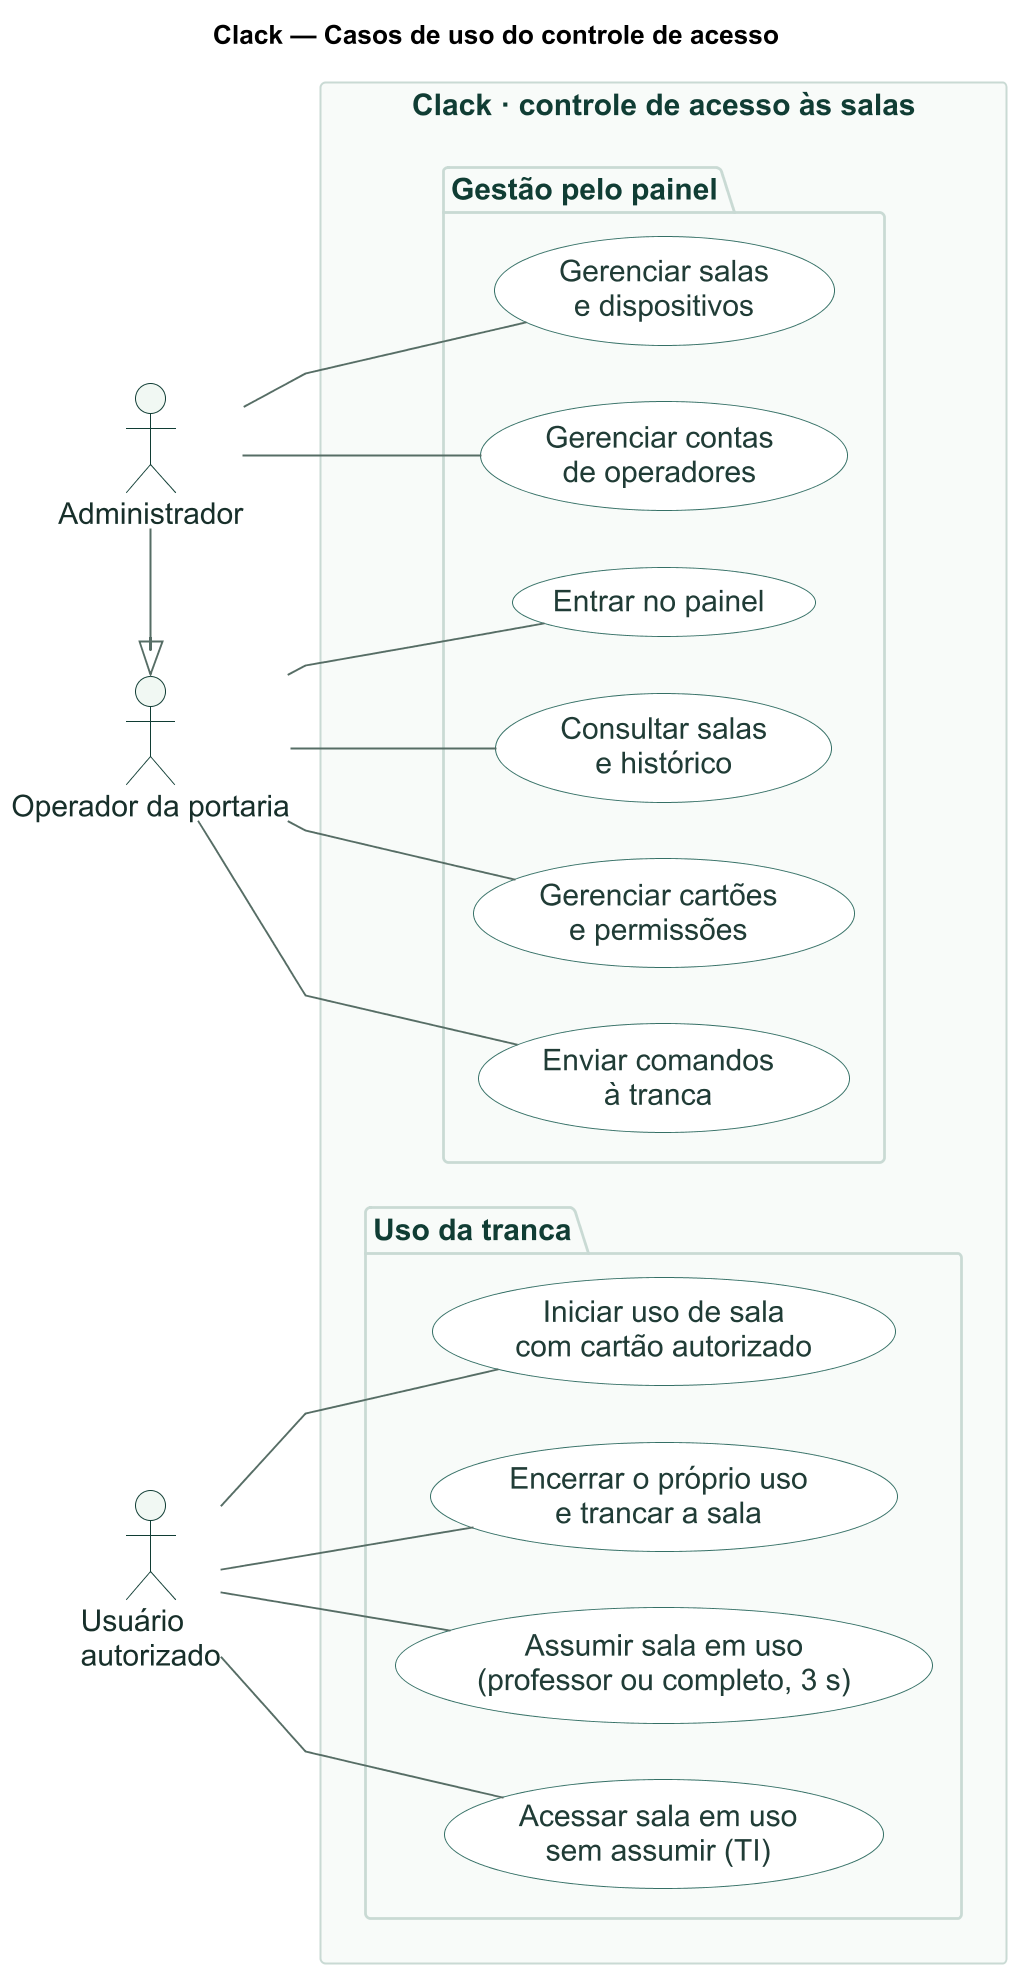
\includegraphics[height=0.77\textheight,keepaspectratio]{figuras/casos-de-uso-clack.png}
  \caption{Casos de uso do controle de acesso às salas no Clack. Fonte: elaboração própria.}
  \label{fig:casos}
\end{figure}

\subsection{Regras de uso da sala}

Uma sala disponível pode ser iniciada por um cartão autorizado conforme seu perfil. A atividade é associada a um responsável; uma nova aproximação do cartão responsável pode encerrá-la e acionar o fechamento. Em uma sala já em uso, a lógica de professor e de perfil completo prevê a transferência de responsabilidade quando o cartão de outra pessoa autorizada é mantido no leitor por três segundos. Uma aproximação curta não deve executar essa transferência nem acionar o servo.

Após a transferência, a nova pessoa responsável pode encerrar a atividade por uma nova aproximação, depois da retirada da etiqueta. A transferência em si não movimenta o mecanismo. A regra também evita que a permanência de uma mesma tag no leitor repita continuamente a ação. Para o perfil de tecnologia da informação (TI), o acesso a uma sala ocupada pode ser registrado sem mudar o responsável anterior, respeitando as condições previstas pelo sistema.

As regras de aluno e limpeza possuem restrições próprias e a forma de atendimento da equipe de limpeza ainda requer confirmação para o cenário institucional. Estados de manutenção e erro bloqueiam decisões normais por cartão. O painel permite intervenções autorizadas, registradas como comandos com prazo e confirmação. A resposta enviada pelo firmware indica que o comando foi processado, não uma medição física da porta.

\subsection{Dados e relacionamentos}

O banco de dados organiza as informações necessárias à gestão e ao registro das ações. A entidade de cartões identifica as pessoas e seus perfis; a de ambientes representa as salas e seu estado. A tabela de permissões associa cartões aos ambientes autorizados, possibilitando que uma pessoa possua acesso a mais de uma sala e que uma sala tenha mais de um cartão autorizado.

Os dispositivos podem ser cadastradores ou trancas e, no esquema atual, a associação de uma tranca a um ambiente é opcional e única. Eventos registram dados como dispositivo de origem, ambiente, sequência e resultado. Comandos relacionam um operador ao dispositivo que receberá a ação; capturas apoiam o cadastramento de cartões, e a auditoria mantém o registro de operações administrativas. A Figura~\ref{fig:er} apresenta uma visão lógica resumida das principais tabelas e chaves.

\begin{figure}[p]
  \centering
  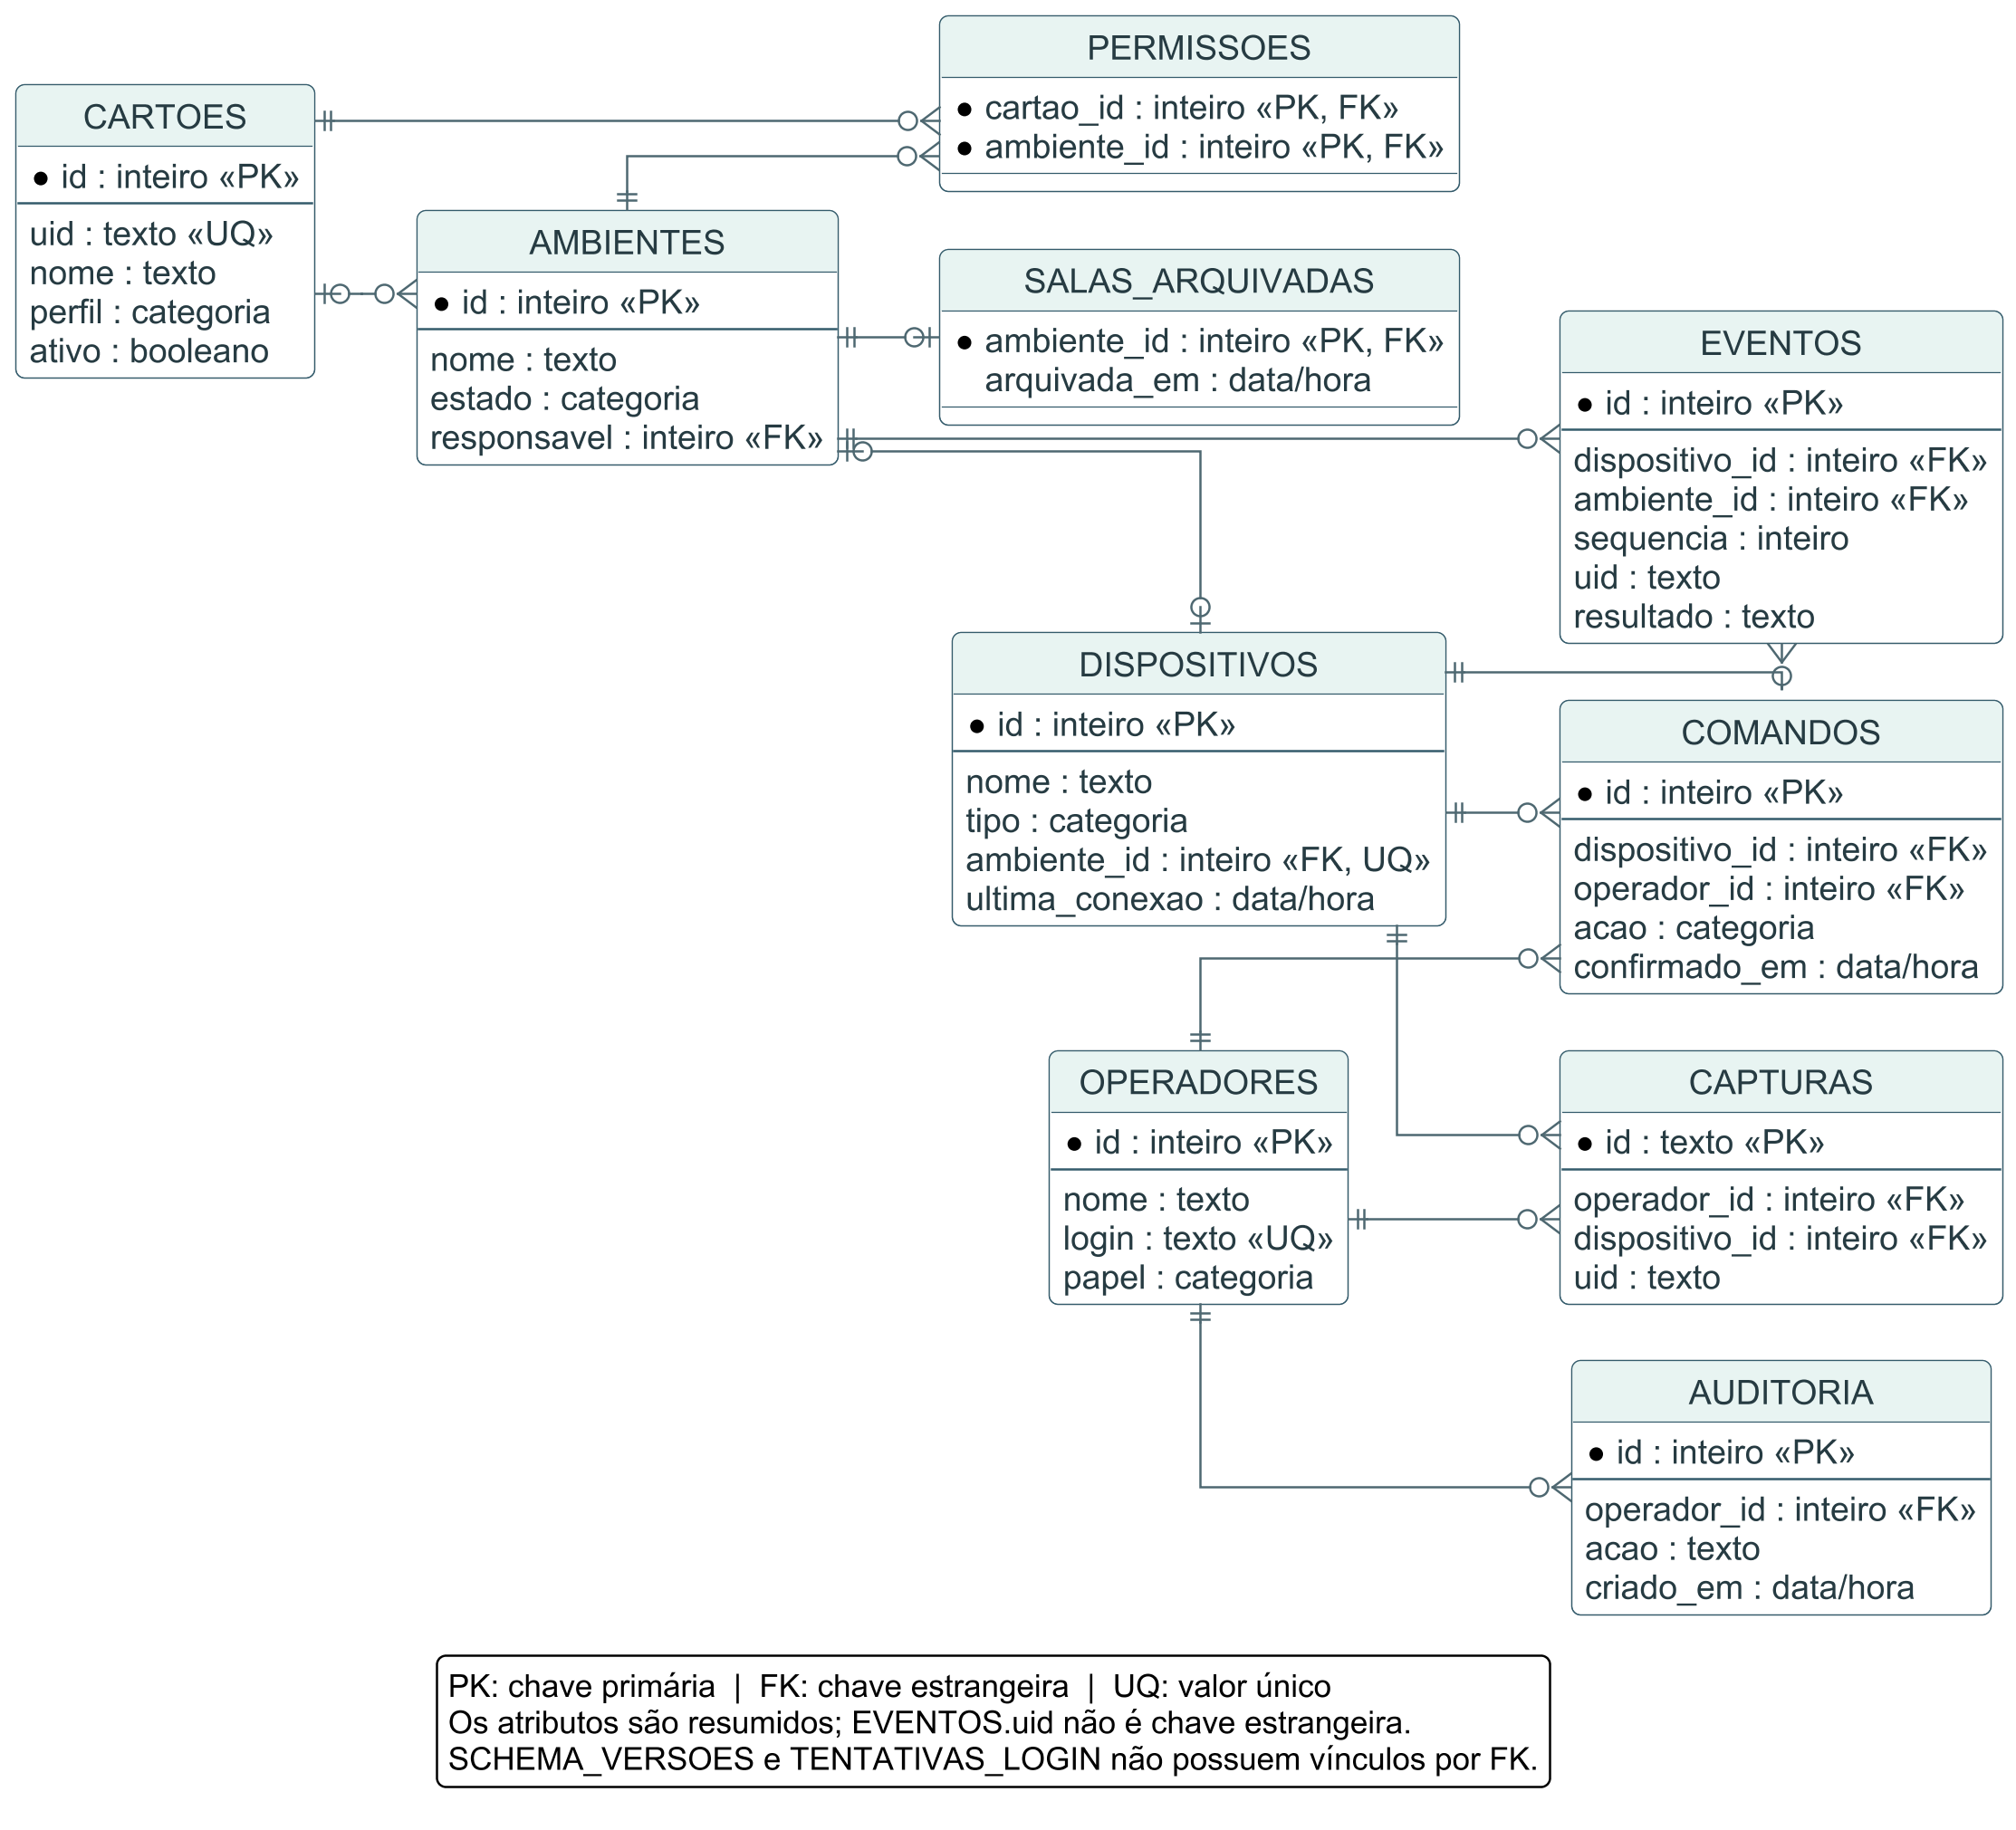
\includegraphics[width=\textwidth,height=0.73\textheight,keepaspectratio]{figuras/modelo-er-clack.png}
  \caption{Modelo lógico resumido das entidades e relações do banco de gestão. Fonte: elaboração própria com base em \texttt{sql/gestao.sql}.}
  \label{fig:er}
\end{figure}

O diagrama apresenta apenas atributos selecionados. A chave composta da tabela de permissões impede duplicar a mesma associação entre cartão e ambiente. Em eventos, a combinação de dispositivo e sequência possui restrição de unicidade, empregada no tratamento de reenvios. O UID armazenado em um evento é um valor de histórico, sem chave estrangeira direta para o cadastro de cartões. As tabelas auxiliares de versão do esquema e controle de tentativas de login não possuem vínculos por chave estrangeira e são descritas na documentação do diagrama.

\subsection{Sincronização e situações de falha}

Ao registrar uma atividade, a tranca atualiza seu estado e acrescenta um evento identificado por uma sequência. Quando há comunicação, envia ao servidor os eventos pendentes e recebe confirmações e atualizações necessárias. A confirmação permite retirar da fila local os eventos reconhecidos, enquanto a restrição de unicidade no banco contribui para evitar registros duplicados em reenvios.

A fila da versão analisada comporta até 64 eventos. Quando esse limite é atingido, a tranca de sala apresenta a condição de histórico cheio e deixa de aceitar novas operações que exigiriam registro até que a sincronização libere espaço. Essa escolha preserva a rastreabilidade esperada, mas limita a duração prática da operação sem comunicação em cenários com muitos usos. A avaliação física do comportamento de perda e retorno de rede na montagem final permanece necessária.

Durante uma tentativa de troca de responsável, o firmware prevê uma sequência luminosa e, após a confirmação local, três piscadas verdes. As luzes têm função de orientar a interação, mas a instalação informada dos LEDs não substitui o registro de um ensaio documentado das cores e dos tempos no protótipo final. A comunicação de rede e a indicação luminosa não comprovam, isoladamente, que o ferrolho se deslocou até uma posição determinada.

\subsection{Interface de gerenciamento}

O painel disponibiliza a visualização de ambientes, seus estados e informações de uso, além de cadastro de cartões, permissões e dispositivos. Uma planta permite identificar as salas por marcadores; os detalhes e as ações disponíveis dependem da conta conectada. Há ainda consulta ao histórico de eventos e registro das intervenções realizadas pelos operadores.

\begin{figure}[htbp]
  \centering
  \fbox{\parbox[c][3.0cm][c]{0.84\textwidth}{\centering\textbf{Imagem pendente}\\Captura do painel com ambientes e dados fictícios}}
  \caption{Exemplo da interface web de gerenciamento do Clack.}
  \label{fig:painel}
\end{figure}

A Figura~\ref{fig:painel} reserva espaço para uma captura da interface em versão identificada, usando dados fictícios ou autorizados. Na interpretação do painel, o estado de comunicação do dispositivo é distinto da ocupação registrada e da posição mecânica da porta. A ausência de contato recente exige diagnóstico e não permite concluir, por si só, a causa da desconexão.

\section{Resultados e discussão}

\subsection{Protótipo e testes funcionais}

O desenvolvimento resultou em firmware para a tranca e para o cadastrador, um servidor de gerenciamento e uma interface para a portaria. Em teste acompanhado da sala 204, em 9 de novembro de 2026, foi observada a regra de transferência: a aproximação rápida de um segundo cartão não alterou o responsável; a permanência da tag por aproximadamente três segundos realizou a transferência sem movimento do servo. Depois da retirada e de nova aproximação, o novo responsável conseguiu encerrar a atividade.

O funcionamento de abertura e fechamento por comandos do painel também foi relatado durante os testes anteriores. Essas observações dizem respeito a uma unidade e a uma versão utilizada na ocasião; não demonstram que todas as funções da versão atual tenham sido validadas em campo. Houve ainda relato de intermitência de leitura no hardware, sem diagnóstico conclusivo. A verificação de fiação, alimentação e leitor continua necessária na montagem final.

As verificações automatizadas da aplicação utilizaram dados descartáveis para exercitar funções de autenticação, permissões, comandos e histórico. Esses testes fornecem evidências sobre o comportamento do software nos cenários executados, mas não comprovam, por si, o funcionamento de uma tranca física nem a resistência do mecanismo instalado em uma porta.

\subsection{Desempenho com 50 trancas simuladas}

No ensaio de carga foram medidas 3.060 requisições ao longo de 60,04 segundos: 500 aberturas, 2.000 consultas periódicas das trancas, 500 fechamentos e 60 consultas ao painel. Não houve respostas classificadas como erro no cenário executado. Ao final, o banco continha os 1.000 eventos esperados, sem divergência detectada nas comparações de estado e responsabilidade realizadas pelo roteiro.

\begin{table}[htbp]
  \centering
  \caption{Tempos de resposta observados no ensaio local com 50 trancas simuladas.}
  \label{tab:desempenho}
  \small
  \begin{tabular}{lrrrr}
    \toprule
    Operação & Requisições & Mediana & P95 & Máximo \\
    \midrule
    Abertura & 500 & 127 ms & 340 ms & 469 ms \\
    Consulta da tranca & 2.000 & 109 ms & 275 ms & 388 ms \\
    Fechamento & 500 & 131 ms & 317 ms & 416 ms \\
    Consulta do painel & 60 & 110 ms & 295 ms & 365 ms \\
    \bottomrule
  \end{tabular}
\end{table}

Conforme a Tabela~\ref{tab:desempenho}, as medianas das operações medidas ficaram entre 109 e 131 ms. O percentil 95, indicado por P95, corresponde ao valor abaixo ou igual ao qual se encontram pelo menos 95\% das medições segundo o método usado no ensaio. As chamadas dos 50 clientes estiveram simultaneamente em andamento em cada uma das 60 rodadas; isso não determina a forma de execução interna das operações no servidor ou no banco.

Os serviços mantiveram os mesmos contêineres e não apresentaram reinícios durante essa execução. O resultado demonstra que o servidor suportou o cenário de carga descrito naquele ambiente, com dados e tempos acelerados. Não é possível concluir, a partir de uma execução de aproximadamente um minuto, que a instalação permanecerá estável durante um dia inteiro de funcionamento real, em rede Wi-Fi ou com histórico de longa duração.

\subsection{Estrutura e estimativa de materiais}

O chassi em PETG demonstra a aplicação de fabricação por impressão 3D ao protótipo, mas sua adequação mecânica não foi estabelecida por testes de carga, número de ciclos ou envelhecimento. A montagem, a orientação de impressão, o encaixe e o comportamento do servo precisam ser documentados em um ensaio próprio antes de qualquer conclusão sobre resistência ou vida útil.

O orçamento de materiais levantado para o projeto estimou R\$ 135,31 para uma tranca e R\$ 99,93 para um cadastrador, em consulta de preços de 19 de novembro de 2026. Esses valores são estimativas de componentes e materiais consumidos; não incluem todos os itens possíveis, frete ou mão de obra, e não representam necessariamente o valor efetivamente pago. Uma comparação econômica com produtos comerciais exigiria critérios e condições equivalentes.

\subsection{Limitações e atendimento dos objetivos}

A implementação da tranca, do cadastrador, do painel e da lógica local atende à etapa de desenvolvimento do protótipo, sujeita à identificação da versão instalada na montagem final. O ensaio de requisições fornece uma avaliação inicial do servidor sob concorrência simulada. A sincronização e as regras de acesso estão presentes no software, mas os cenários de interrupção e recuperação de rede ainda precisam de evidência física com o conjunto final.

O objetivo de investigar a resistência mecânica permanece em aberto, assim como a avaliação de usabilidade e impacto com docentes e equipe de limpeza. Não foram localizados registros suficientes para apresentar participantes, tarefas executadas ou resultados dessa avaliação. Também não houve avaliação formal que permita afirmar conformidade integral com a LGPD ou comprovar resistência a clonagem de cartões e interceptação de tráfego.

Essas limitações orientam os próximos testes: realizar uma sequência documentada de operações com cartões autorizados e não autorizados, observar a tranca após interrupção da rede, verificar o histórico depois da reconexão e medir o tempo completo entre leitura, movimento e atualização do painel. Para avaliar o servidor, é necessário repetir a carga por períodos mais longos e incorporar rede e dispositivos físicos na medida em que estiverem disponíveis.

\section{Conclusão e trabalhos futuros}

O Clack reúne uma tranca eletrônica baseada em ESP32 e RFID, um cadastrador e uma aplicação web para o controle de ambientes e permissões. A arquitetura desenvolvida permite a tomada de decisão com dados locais e a posterior sincronização com o servidor, preservando a distinção entre perda de comunicação e falta de energia. O teste de software com 50 trancas simuladas registrou as respostas e os eventos esperados no cenário acelerado descrito.

Os resultados são iniciais e não demonstram implantação institucional concluída. Como continuidade, são necessários testes físicos da versão final, avaliação mecânica, investigação da leitura intermitente e observação do uso por docentes e equipe de limpeza. Recomenda-se também aperfeiçoar a proteção das credenciais e do tráfego, avaliar a política de atualização das permissões e realizar uma análise de privacidade compatível com o contexto de uso.

A integração com horários de aula, a importação de tabelas e uma alimentação de contingência permanecem possibilidades futuras. A conclusão sobre a contribuição operacional do sistema dependerá de uma avaliação em situação real, com procedimento e resultados registrados.

% Entradas do TCC I preservadas provisoriamente sem atribuir a elas afirmações
% que ainda não foram verificadas na fonte primária. Conferir antes da entrega.
\nocite{cruzjunior2024,fornaciari2023,ifsulregulamento}
\clearpage
\bibliographystyle{sbc}
\bibliography{referencias}

\end{document}
